\section*{Results}

\subsection*{Population structure and genetic diversity}
\jri{shortened section title, this ok?}
Founder inbreds and samples from cycles 0, 4, 8, 12, and 16 were genotyped at 39,258 SNPs that passed a set of quality filters and could be assigned collinear genetic and physical map positions (See Materials and Methods for details). 
Change in population structure throughout the Iowa RRS experiment can be observed visually by a principal component analysis (PCA). 
A joint analysis of individuals from all the selection cycles (Figure \ref{fig:pca}) clearly separates the BSSS and BSCB1 populations along the first axis of variation, with increasing separation as the experiment progressed. 
The second axis of variation primarily separates the cycles from one another within each population. 
There is no separation between the founders of the two populations, but at cycle 0, the BSSS population shows more divergence from the founders than does BSCB1. 
This could be due to drift during either the population’s construction or subsequent maintenance. 
Structure continued to develop within each population over the course of the experiment. 
There is an especially wide gap between cycles 4 and 8, which correlates with the addition of an extra generation of self-pollination prior to selection at each cycle. 
The distance between cycles then decreases dramatically after cycle 8, and corresponding to the increased effective population size (See Materials and Methods).

%%%%%%%%%%%%%%%%%%%%%%%%%%%%%%%%%%%%%%%%%% FIGURE
\begin{figure}[tb]   
  \begin{center}
   \vspace{-0mm}
   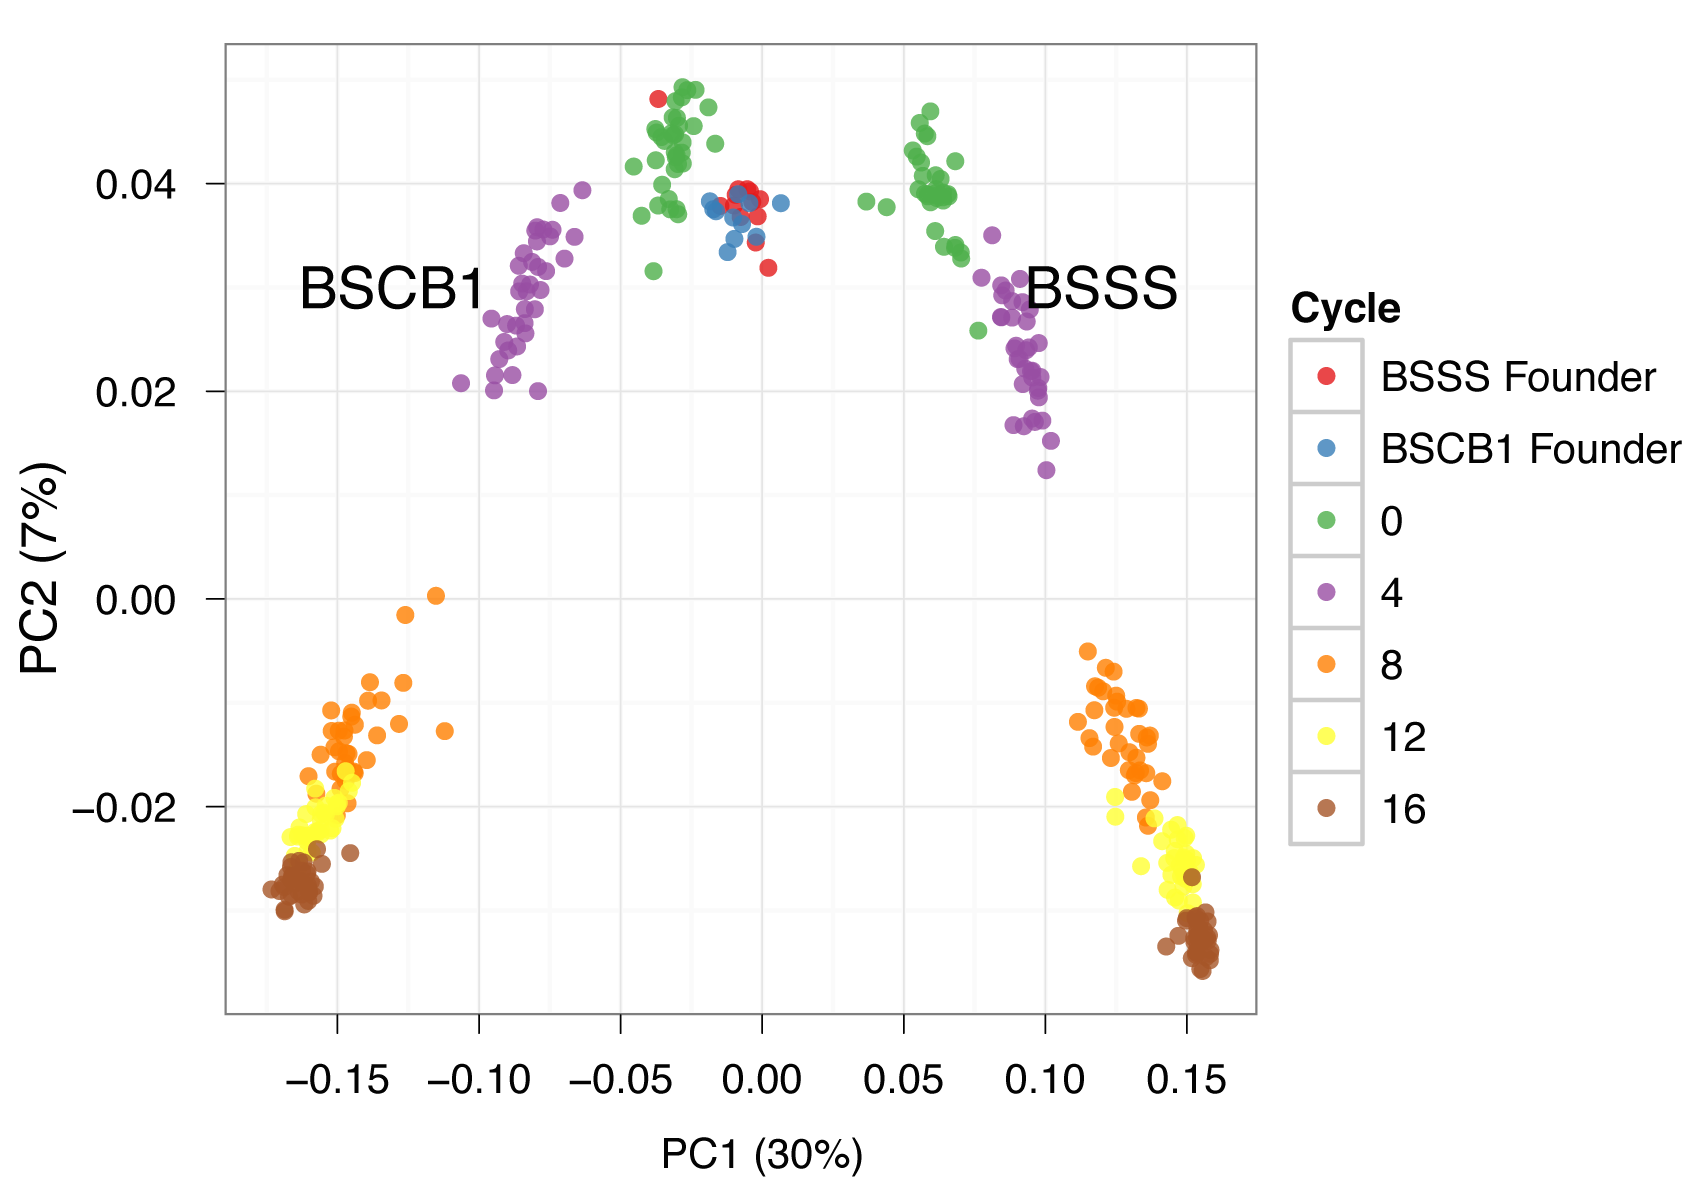
\includegraphics[width=0.5\textwidth]{fig1}
   \renewcommand{\baselinestretch}{0.9}
   \vspace{-3mm}
   \caption{Principal component analysis of the SNP data from Iowa RRS. The axes represent the first two eigenvectors from an analysis of cycles 0-16, with projection of the founder lines onto the vector space. The variation explained by each eigenvector is given in parentheses on the axes. The populations steadily diverge at increasing cycles, with less distinction visible between the founder groups. The comparatively large distance between cycles 4 and 8 corresponds to a switch from one to two generations of selfing at each cycle. The smaller separation between cycles 8-16 corresponds to an increase in effective population size from ten to twenty. The BSSS cycle 0 population has drifted away from the BSSS founders, despite the absence of intentional selection during the creation and maintenance of cycle 0.
} 
\vspace{-6mm}
    \label{fig:pca}
  \end{center}
\end{figure}
%%%%%%%%%%%%%%%%%%%%%%%%%%%%%%%%%%%%%%%%%% FIGURE

No new genetic material was intentionally introduced into either population after the experiment's inception, so the substantial increase in genetic distance could only arise from the loss of genetic diversity within each population. 
Consistent with previous studies of the Iowa RRS, genome-wide genetic diversity (expected heterozygosity, H) decreases steadily across cycles of selection in both populations (Figure \ref{fig:decline}). 
\jri{need a citation here of "previous studies"?}
The loss of heterozygosity is smaller when the two populations are considered together, indicating the loss of different alleles within BSCB1 and BSSS. 
This genetic differentiation is reflected by the tenfold increase in $F_{ST}$ between the founder lines and the populations at cycle 16. 

%%%%%%%%%%%%%%%%%%%%%%%%%%%%%%%%%%%%%%%%%% FIGURE
\begin{figure}[tb]   
  \begin{center}
   \vspace{-0mm}
   \includegraphics[width=0.5\textwidth]{fig2}
   \renewcommand{\baselinestretch}{0.9}
   \vspace{-3mm}
   \caption{Heterozygosity and $F_{ST}$ across cycles. $H$ (left panel) and $F_{ST}$ (right panel) plotted as a function of selection cycle in each population.
} 
\vspace{-6mm}
    \label{fig:decline}
  \end{center}
\end{figure}
%%%%%%%%%%%%%%%%%%%%%%%%%%%%%%%%%%%%%%%%%% FIGURE

We noticed an irregular increase in the number of polymorphic markers between BSSS cycles 4 and 8 (Table S2). 
All of these newly polymorphic markers were present at extremely low frequency and were spread among various individuals. 
This may represent a series of minor alleles that were not captured in our sample of cycle 4 individuals and thus appeared to ‘resurface’ at cycle 8. 
Alternatively, the pattern may be the result of minor contamination at some point in the population’s history. 
It was observed that an allele of the sugary gene associated with sweet corn appeared in the population at this time (O.S. Smith, personal communication), suggesting contamination may be the cause. 
However, the low frequency of the ‘new’ alleles (typically only one or two alleles out of 72 possible in 36 diploid samples) means their effect on population diversity is minimal.  
We did not attempt to incorporate this contamination into our simulation approaches, as it only makes our tests for low heterozygosity slightly more conservative.

\subsection*{Fixation of large genomic regions}
Figure \ref{fig:heterotic} shows heterozygosity varying along the genome across cycle 16 of each population. 
Of particular note are extremely large pericentromeric regions of zero or near-zero heterozygosity spanning tens of megabases. 
These regions experience low rates of meiotic recombination, which creates an expanded physical map relative to their genetic length \citep{ganal2011a-large}. 
In general, the majority of fixed haplotype segments are small (<2 cM) in genetic space regardless of their physical size; one exception is 7 cM region on chromosome 1 in the BSCB1 population. 

%%%%%%%%%%%%%%%%%%%%%%%%%%%%%%%%%%%%%%%%%% FIGURE
\begin{figure}[tb]   
  \begin{center}
   \vspace{-0mm}
   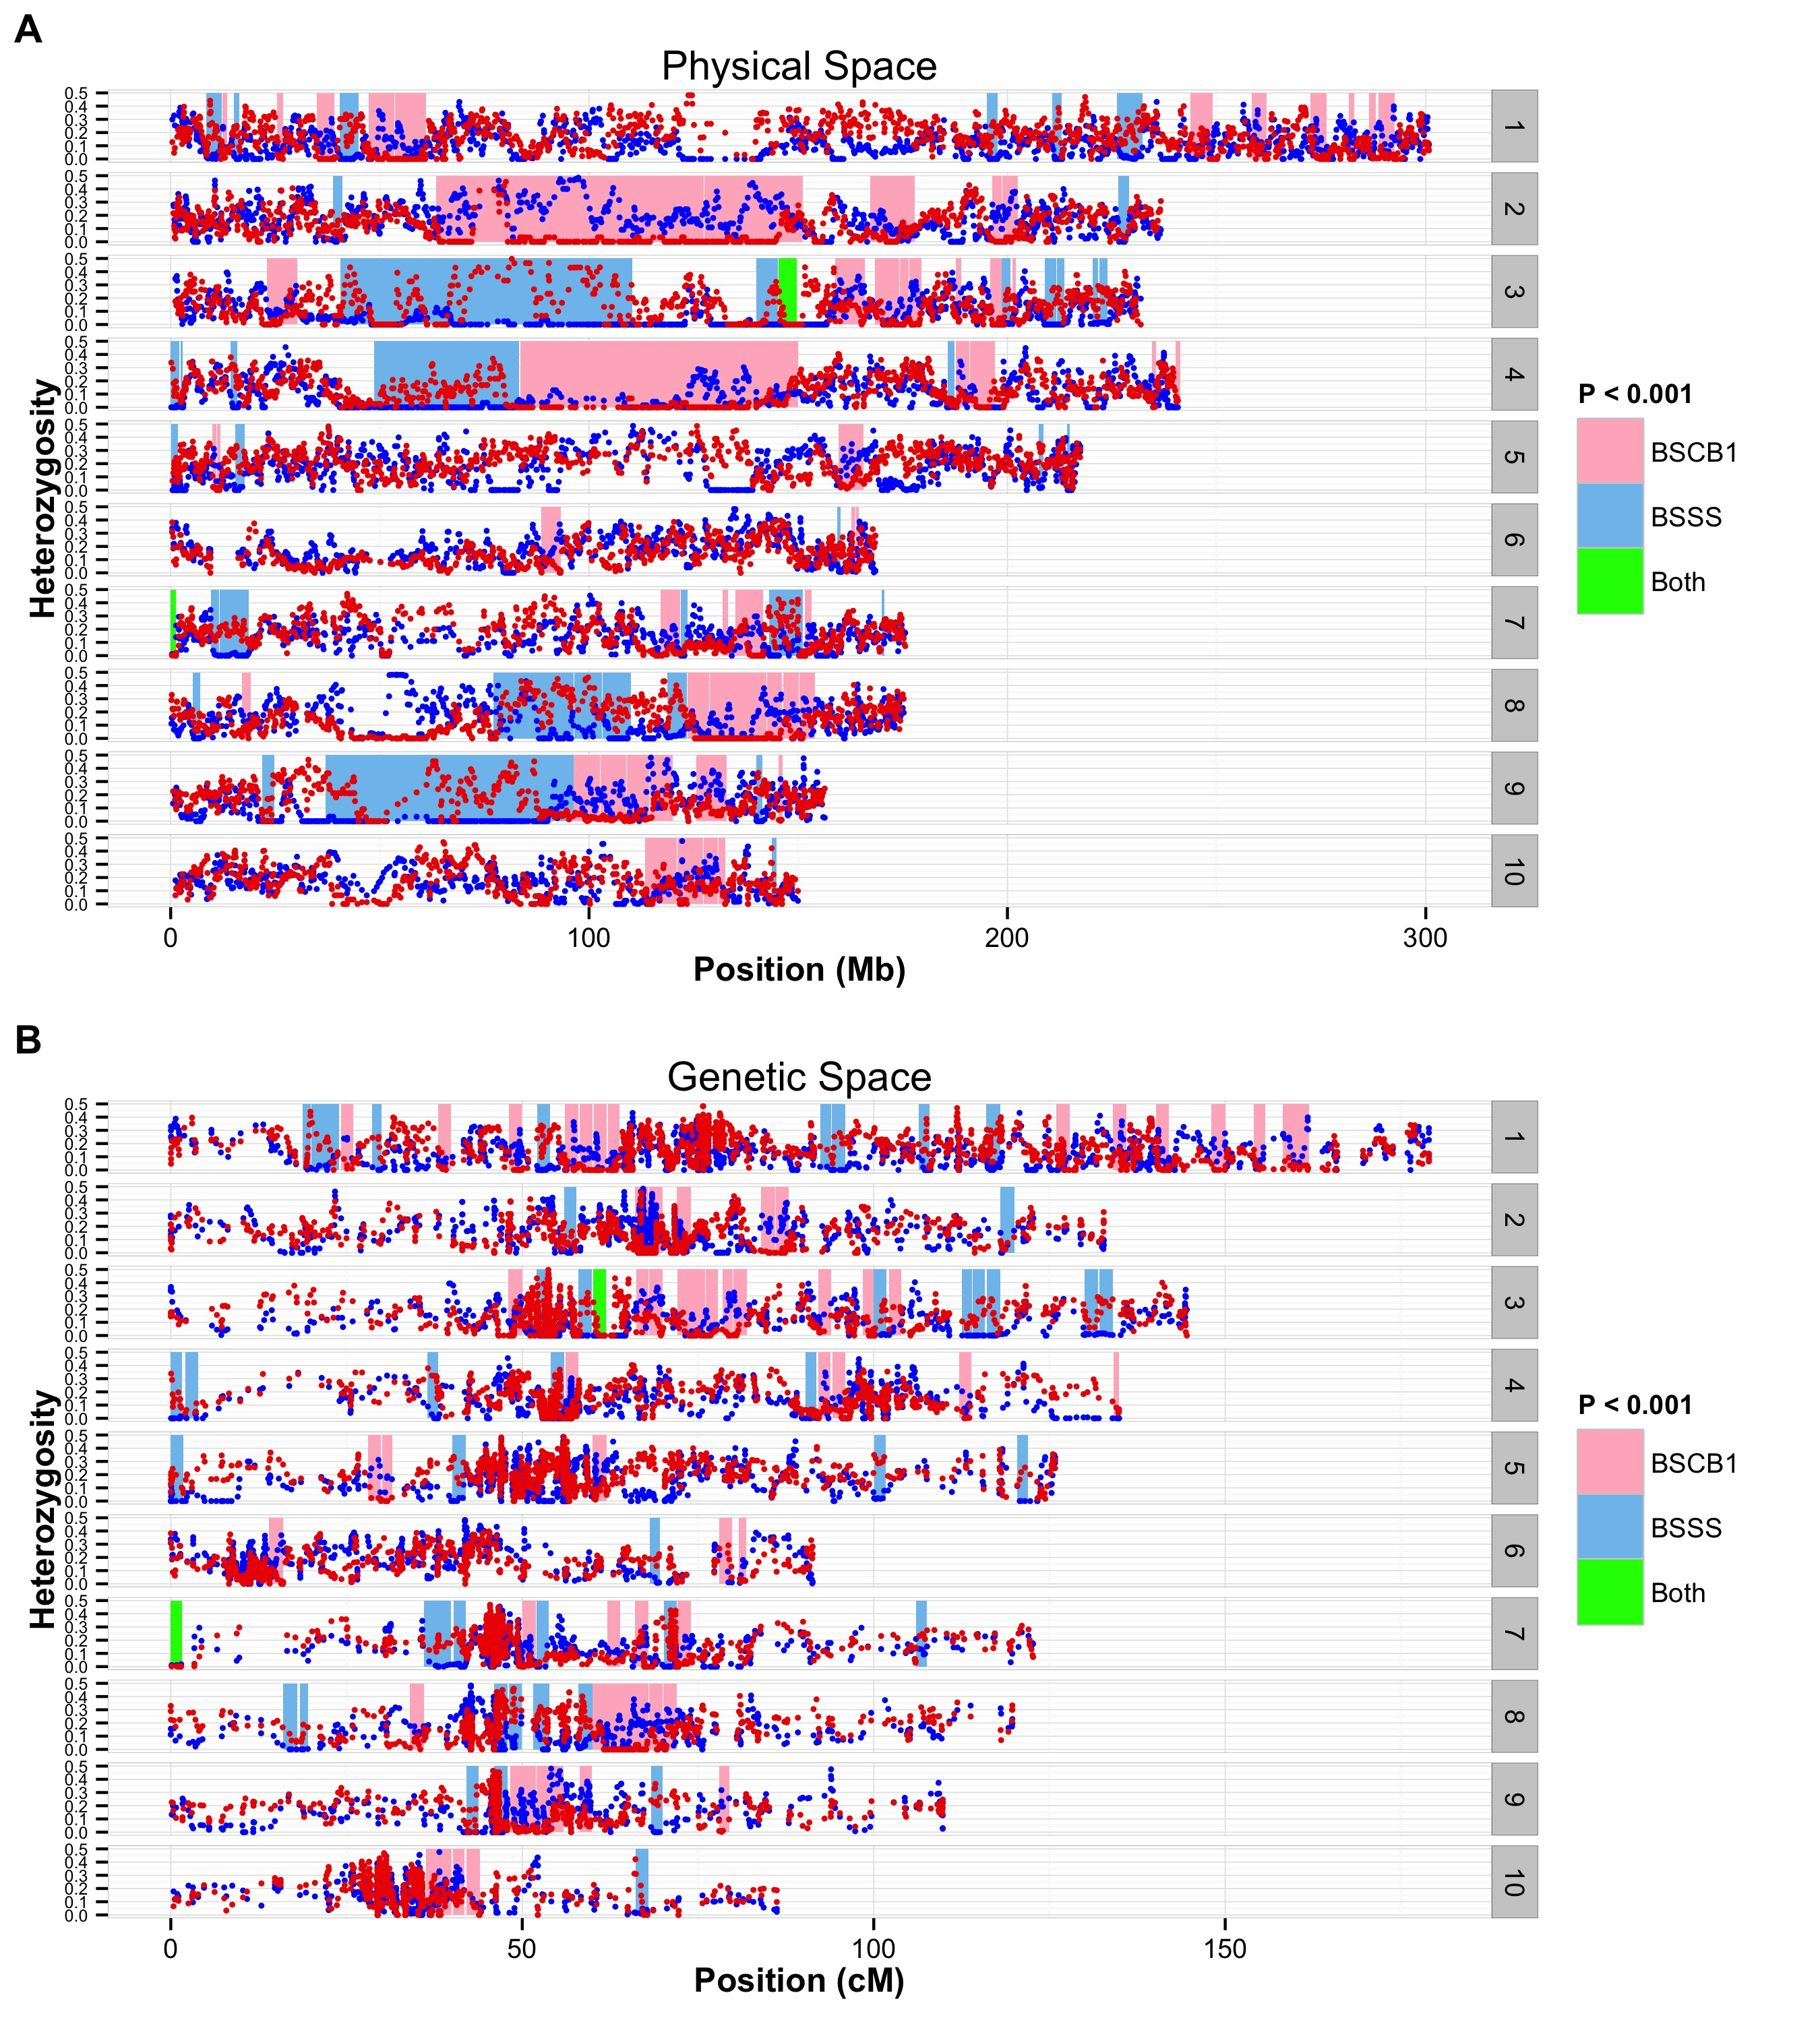
\includegraphics[width=0.5\textwidth]{fig3}
   \renewcommand{\baselinestretch}{0.9}
   \vspace{-3mm}
   \caption{ Heterozygosity ($H$) at cycle16 across all ten chromosomes in each population.  $H$ is calculated on 15-marker sliding windows with 5 marker steps. Each point is plotted at the midpoint of the 15-marker window. 
} 
\vspace{-6mm}
    \label{fig:heterotic}
  \end{center}
\end{figure}
%%%%%%%%%%%%%%%%%%%%%%%%%%%%%%%%%%%%%%%%%% FIGURE

The sheer physical size of the pericentromeric regions yields extremely high marker density on the genetic map, allowing for clear resolution of haplotype phasing and recombination breakpoints. 
To further examine the fixation in these regions, we computationally imputed haplotype phase in the BSSS and BSCB1 populations and used the phased data to track haplotype frequencies and founder of origin. 
In most cases, these fixed haplotypes can be traced back to single founder inbreds. 
For example, in BSSS, a 60 Mb (1.2 cM) region of chromosome 9 became fixed by cycle 12 (Figure \ref{fig:genphys}) and traces back to the founder Os420. 
In BSCB1, a 60 Mb (0.7 cM) region became fixed on chromosome 4 and traces back to A340 (Figure \ref{fig:genphys2}). \jri{should figures 4 and 5 be made into a single 4-panel figure?}
Table \ref{tab:fix} gives a summary of the large genomic regions that have become fixed or nearly fixed by cycle 16. 
These regions represent blocks of linked loci that show no evidence of recombination since at least the development of the founding inbred lines in the 1920’s and 1930’s.
	
%%%%%%%%%%%%%%%%%%%%%%%%%%%%%%%%%%%%%%%%%% FIGURE
\begin{figure*}[tb]   
  \begin{center}
  % \vspace{-0mm}
   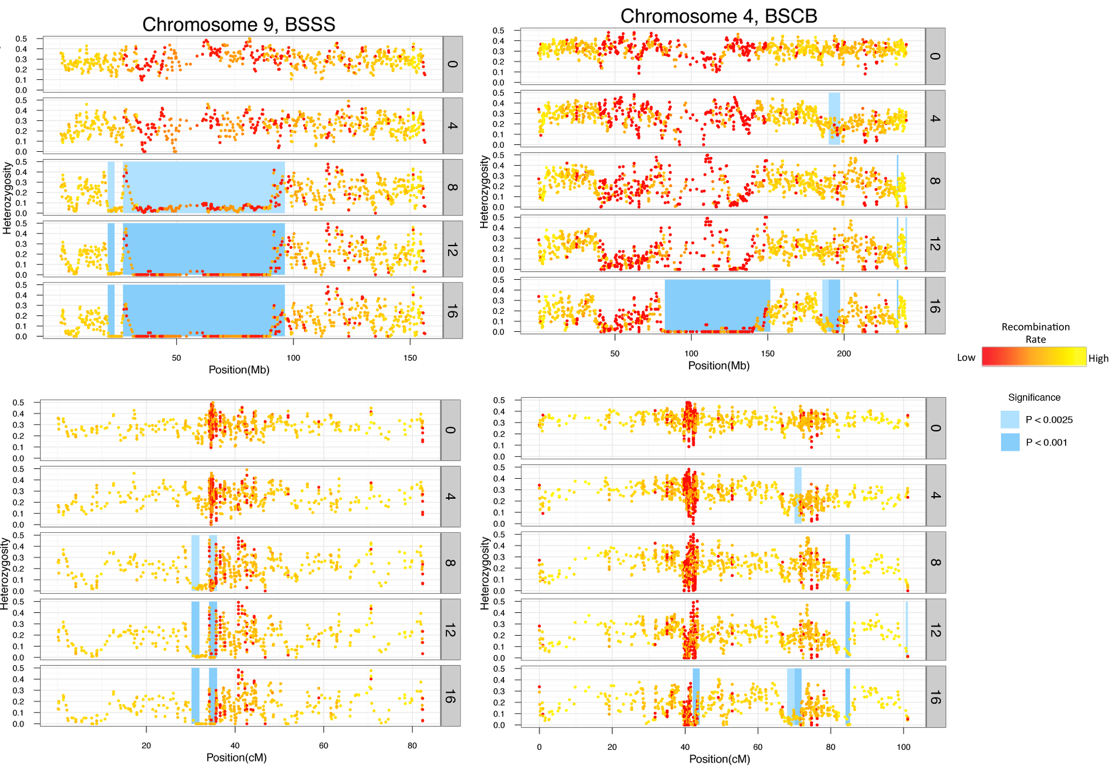
\includegraphics[width=\linewidth]{fig45}
 %  \renewcommand{\baselinestretch}{0.9}
 %  \vspace{-3mm}
   \caption{Heterozygosity ($H$) across chromosomes 9 (left) and 4 (right) in each cycle of BSSS plotted on the physical (top) or genetic (bottom) map. H is calculated on 15-marker sliding windows, with 5 marker steps between each calculation. Each data point is color-coded based on a linear transformation of recombination rate (red = low recombination rate). Shaded regions represent 2 cM windows found to have heterozygosity values significantly lower than expected by simulation at a given cycle. Light shading denotes significance at P < 0.0025, whereas the darker shading represents significance at P < 0.001. Comparing the physical and genetic maps reveals that the regions of fixation are extremely small genetically, but some contain much of the physical content of the chromosome.
} 
\vspace{-6mm}
    \label{fig:genphys}
  \end{center}
\end{figure*}
%%%%%%%%%%%%%%%%%%%%%%%%%%%%%%%%%%%%%%%%%% FIGURE	



%%%%%%%%%%%%%%%%%%%%%%%%%%%%%%%%%%%%%%%%%% FIGURE
%\begin{figure}[tb]   
%  \begin{center}
%   \vspace{-0mm}
%   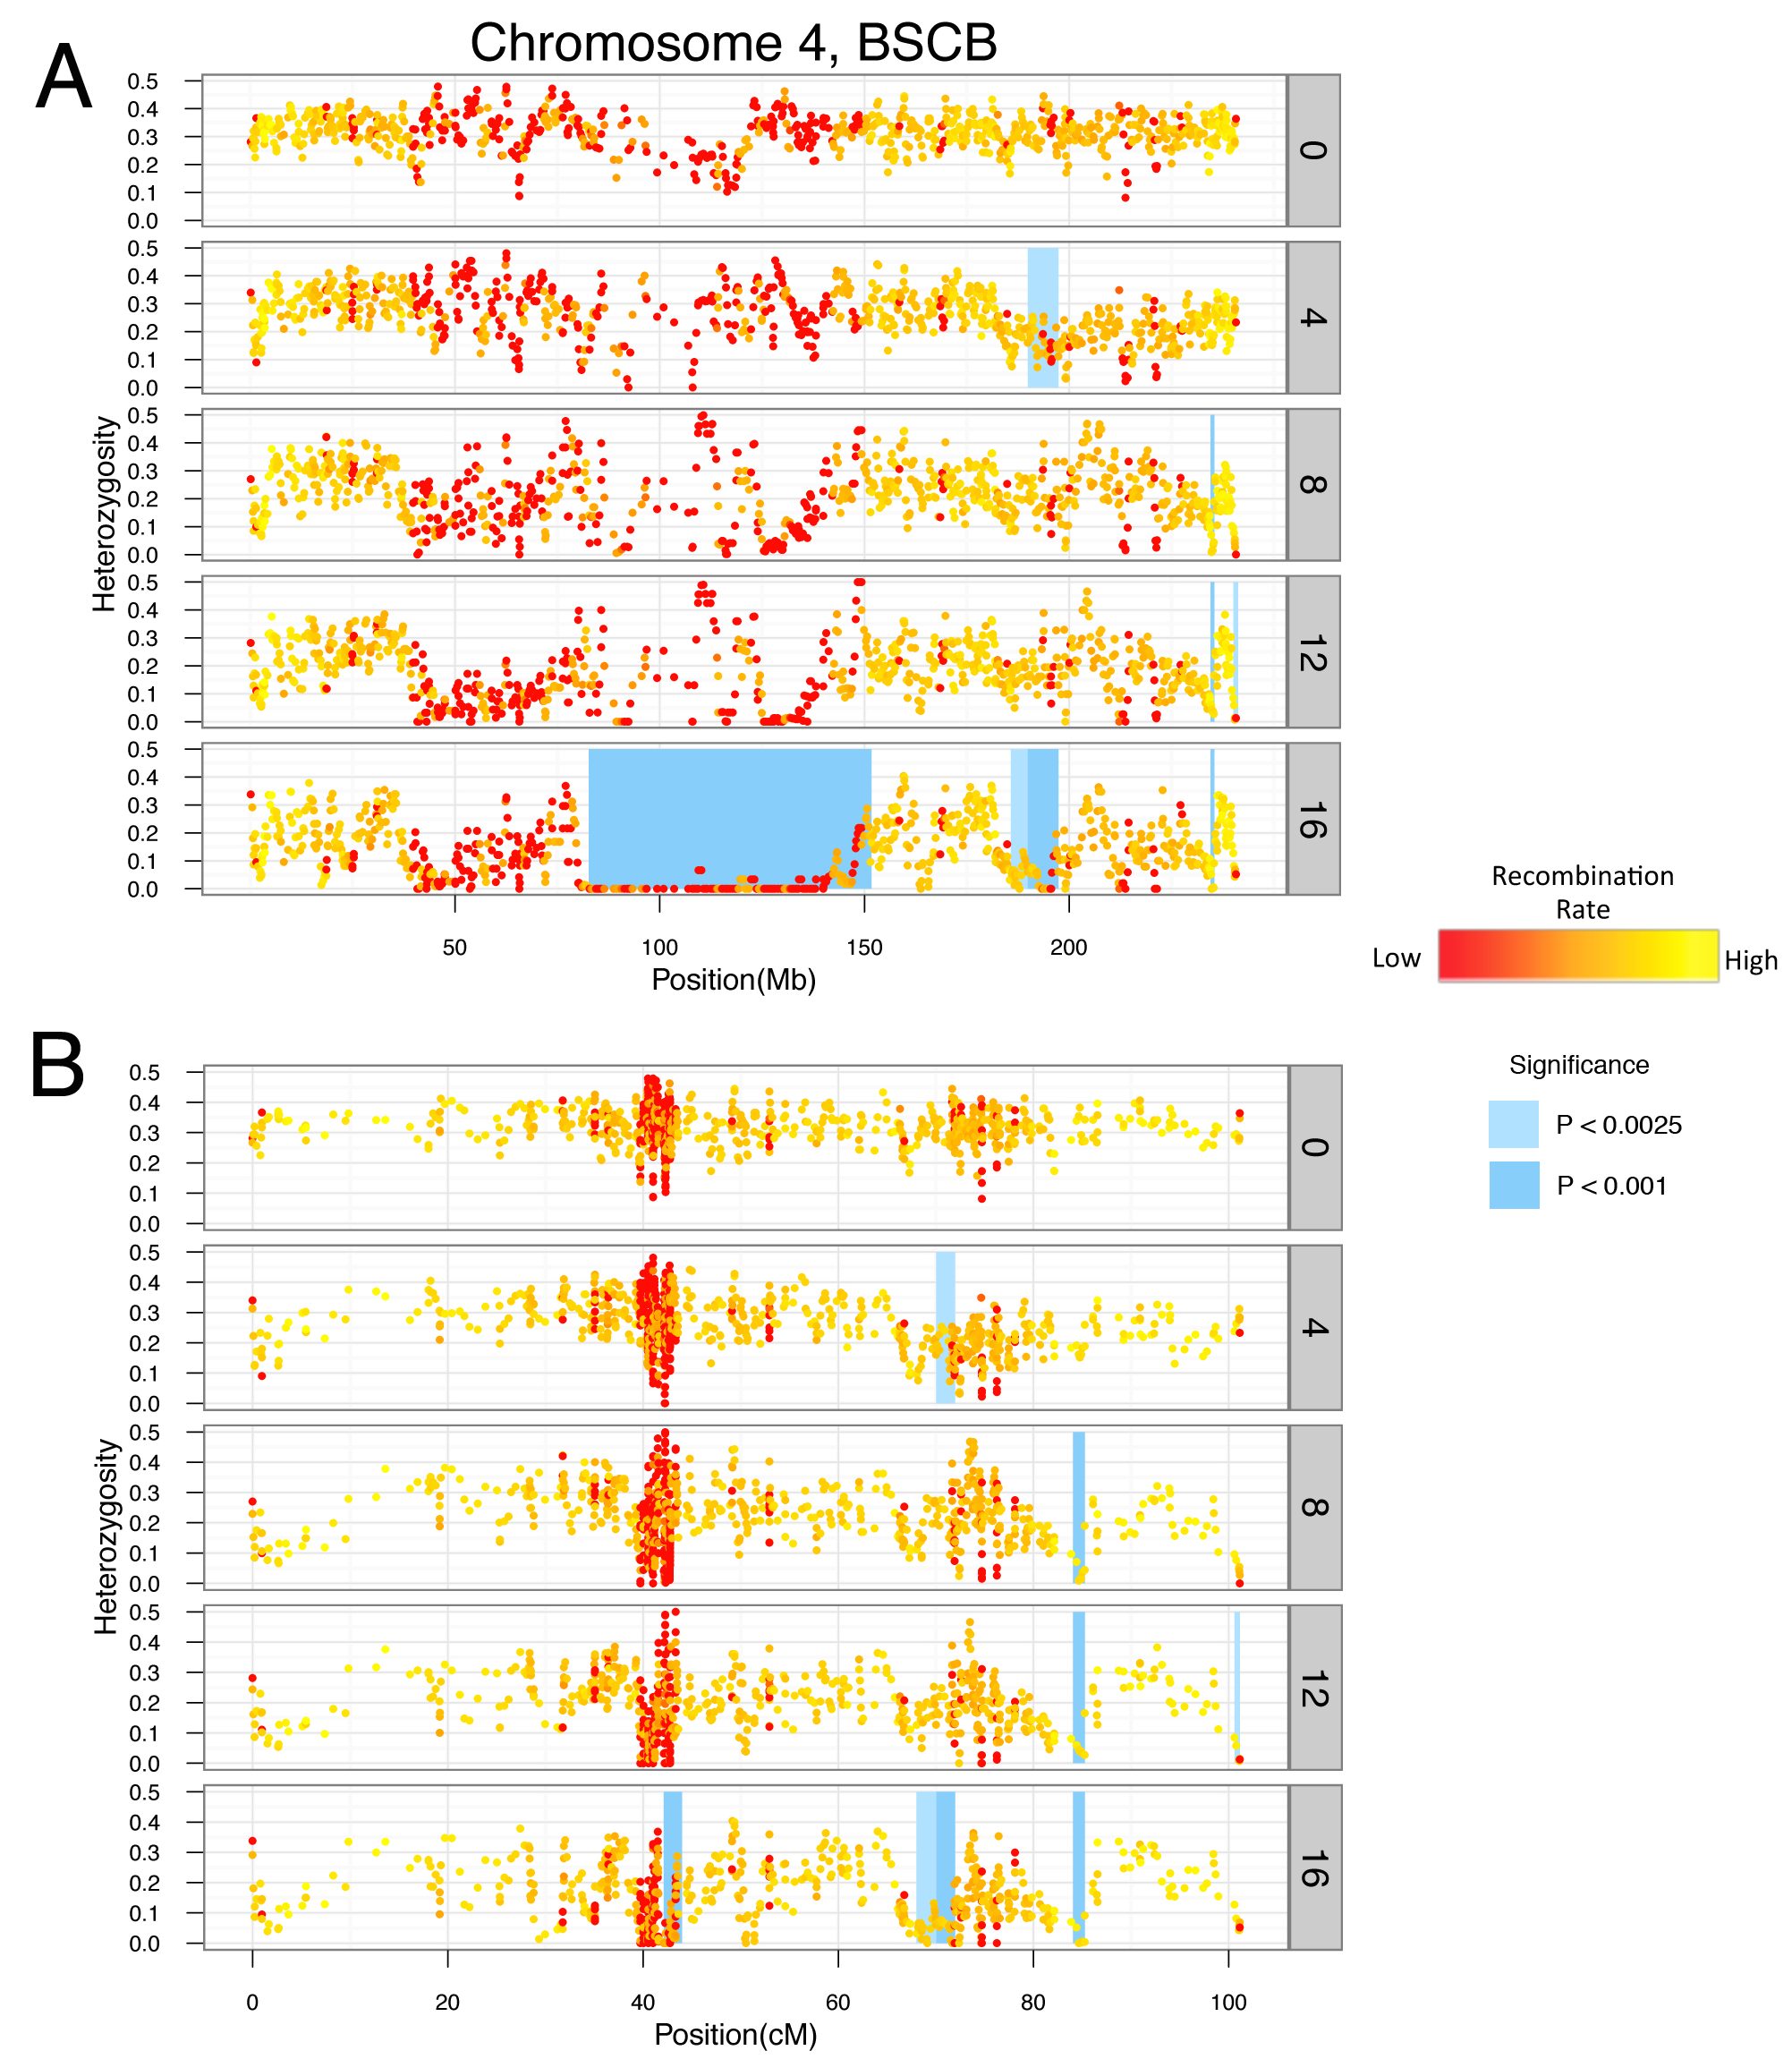
\includegraphics[width=0.5\textwidth]{fig5}
%   \renewcommand{\baselinestretch}{0.9}
%   \vspace{-3mm}
%   \caption{Heterozygosity ($H$) across chromosome 4 in each cycle of BSCB1 plotted on the physical (A) or genetic (B) map.  $H$ is calculated on 15 marker-sliding windows, with 5 marker steps between each calculation. Each data point is color-coded based on a linear transformation of recombination rate (red = low recombination rate). Shaded regions represent 2 cM windows found to have heterozygosity values significantly lower than expected by simulation at a given cycle. Light shading denotes significance at P < 0.0025, whereas the darker shading represents significance at P < 0.001.
%} 
%\vspace{-6mm}
%    \label{fig:genphys2}
%  \end{center}
%\end{figure}
%%%%%%%%%%%%%%%%%%%%%%%%%%%%%%%%%%%%%%%%%% FIGURE

\subsection*{The role of genetic drift}
There is clear evidence of phenotypic improvement in response to selection in the Iowa RRS populations (Smith, 1983; Keeratinijakal and Lamkey, 1993; Schnicker and Lamkey, 1993; Holthaus and Lamkey, 1995; Brekke et al., 2011a; Brekke et al., 2011b; Edwards, 2011) and large changes in genetic structure indicated by molecular markers. 
A central issue for these maize populations and others like them is whether the changes observed at the molecular level are caused directly by selection on phenotype, or indirectly due to the genetic drift that selection imposes through inbreeding and small effective population sizes. 
To gauge the roles of selection and drift, we conducted simulations of the crossing and selection schemes used in the RRS experiment, with genetic recombination modeled on a framework map of a cross between B73 (a BSSS derived line used to construct the reference genome) with Mo17 (an inbred with some co-ancestry to both the BSSS and BSCB1 founder germplasm)\citep{gerdes1993compilation}\citex{Lee et al., 2002}. 
Selections were executed at random in each simulation, so the patterns observed across simulations represent the expected distribution of effects caused only by recombination and genetic drift. 
We conducted 10,000 simulations, sampled individuals from each cycle equal in number to the observed samples, measured heterozygosity, and compared the results to the observed data. 	
	
Averaged across the genome, the vast majority of the reduction in diversity observed in both populations can be attributed to genetic drift. 
Nonetheless, do observe deviations from the simulated values (Figure S1). 
The observed data show higher than expected heterozygosity at cycle 4, suggesting selection for heterozygosity in early cycles, a deviation from simulated and actual breeding practices, or an under-sampling of the diversity present in the original cycle 0 populations. \jri{where is this excess of diversity? if it's all pericentromeric can we argue for the first hypothesis?}
As the cycles progress, heterozygosity falls more rapidly than expected in both populations, and the observed values at cycle 16 are significantly lower than the simulated data.  
Simulations across a number of different marker densities were consistent with this result (data not shown). 

To examine the behavior of specific regions, we also calculated the observed and simulated results for each 2 cM segment of the genome. 
The dynamics observed across most of the genome are largely insensitive to changes in window size (we tested from 2-4 cM, data not shown), and are consistent with strong genetic drift imposed by selection practices. \jri{did we test smaller regions? not enough markers?}
A subset of loci were flagged as significant, and these loci almost always overlapped regions of fixation or near-zero heterozygosity in one population. 
However, in these regions the values obtained by simulation are often quite low, such that the extreme simulated values sometimes lie only a few percentage points away from the observed value (Supplementary File S2), indicating that drift alone can explain most of the drop in diversity. 

Since the population size of the Iowa RRS is small (10-20), many biallelic SNPs should fix by chance regardless of their starting minor allele frequencies. The deviation from simulation arises not from changes in allele frequencies per se, but rather from the fixation of linked markers across larger than expected genetic distances. 
The validity of significance cutoffs therefore depend on the accuracy of our genetic map, and the maize genetic map is known to vary among genetic backgrounds across short genetic distances (< 5cM) (McMullen et al., 2009). \jri{need to cite either \citep{bauer2013intraspecific} who shows there's lots of variation or maybe also \citep{rodgers2015recombination} who argues it's stable (but stable vs. variable is somewhat subjective}
Deviations of the observed and simulated results could be due to selection, variation / inaccuracy in the genetic map, or a combination of these factors. 

To explore the roles of selection and drift independent of the genetic map, we returned to the large regions of fixation in the centromeres which showed no recombination across the full RRS experiment. 
Given the lack of recombination, each of these regions can be analyzed by the simulation of a single locus, and the high density of markers allows the clear resolution of the individual haplotypes. 
We used the computationally phased data to measure the frequency of the fixed haplotype at each cycle, and assessed the probability of observing the fixation event given the initial frequency. 
The BSSS chromosome 9 haplotype fixed at cycle 16 was at low frequency at cycle 0 (7 out of 68 haplotypes), but increased rapidly in frequency by cycle 8 (66 out of 70 haplotypes). 
Simulation of the haplotype as a single locus in the RRS experiment produces this increase in frequency in only 3.9\% of 1000 independent simulations, whereas the haplotype was lost in over 80\% of the simulations. 
In BSCB1, a 30 Mb, 1.6 cM region of chromosome 2 became nearly fixed by cycle 8 (67/70) despite a prevalence of 4/72 at cycle 0, which occurred 1.5\% of the time by simulation. 
Although these results suggest that selection may have pushed these haplotypes to fixation, the fact that fixation of such a rare haplotype still occurred in some simulations speaks to the strong genetic drift imposed upon the BSSS and BSCB1 populations. \jri{do you think we need to do more to explain here or above? in the previous paragraph we argue biallelic loci should fix by chance regardless of starting allele freq.}  
Interestingly, each of these two genomic regions harbored a different cycle 0 haplotype at higher frequency, but these higher-frequency haplotypes were subsequently lost within the RRS population. 
In other cases, the haplotypes which eventually fixed were at moderate frequency in the cycle 0 populations and drift to fixation in the majority of simulations.


\renewcommand{\arraystretch}{1.1}
\begin{table}[tb]

\begin{center}
\caption{Ancestry of haplotypes fixed in the cycle 16 population.}
  \textbf{}\\[-2mm]
{\fontsize{6}{9}\sf
\begin{tabular}{llllll}

Population &	 Chr.& Interval (cM) & Interval (Mb) &	Founder & Derived Lines \\
 \hline
BSSS &3	&40.2-41.4	&67.7-123	&CI187-2&	B94  \\
BSSS&	3	&43-48.5&	129.2-157.1	&NDa	&B89, B94 \\
BSSS	&4	&39.7-42.1	&39.9-82.7&	CI187-2	&B89, B94, B67, B72, B39, B43\\
   
 &  &  &  &  &   \\ 
    \hline
    \end{tabular}
    \label{tabfix}
}
\end{center}
\end{table}
\renewcommand{\arraystretch}{1}






%BSSS	
%
%
%BSSS	9	30.6-33.5	20.8-26.6	Oh7b	B89, B94, B43, B17, B72, B84, B67
%BSSS	9	34.3-35.6c	30.8-90.4c	Os420	B89, B94
%BSCB1	2	50.2-51.8	80.6-114.5	CC5	B90, B91, B95, B97, B99
%BSCB1	4	42.1-42.8	82.7-140	NDa	B90, B95, B97
%BSCB1	8	46.1-50.7	125.1-145.6	P8	B90, B97, B91, B99, B54
%
%a ND = Not Determined (Either a recombinant haplotype or originates from an un-genotyped founder)
%
%b Although Oh7 is a BSCB1 founder, it is a descendant of CI.540, an un-genotyped BSSS founder. BSSS segments matching Oh7 presumably derive from CI.540
%
%c  Founders Ind_B2 (BSSS), CI187-2 (BSSS), R4 (BSCB1), and I205 (BSCB1) are all IBD at this region of chromosome 9




